% =============================================================================
%  Figure: the identity ON/OFF parity experiment + per-connector OFF technique
%  ---------------------------------------------------------------------------
%  Standalone-compilable:   pdflatex figure-identity-onoff-parity.tex
%  To include in the thesis: move into thesis-latex/figures/ and either
%    \includegraphics{figures/figure-identity-onoff-parity.pdf}   (compiled PDF), or
%    \input{figures/figure-identity-onoff-parity}  inside a tikzpicture-free figure env
%    (the body below is one tikzpicture; strip the standalone wrapper to \input it).
%  Grayscale-friendly (works in print): ON identity = gray fill, OFF identity = dashed.
% =============================================================================
\documentclass[border=6pt]{standalone}
\usepackage{lmodern}
\usepackage{tikz}
\usetikzlibrary{positioning, calc, arrows.meta, decorations.pathreplacing}

\begin{document}
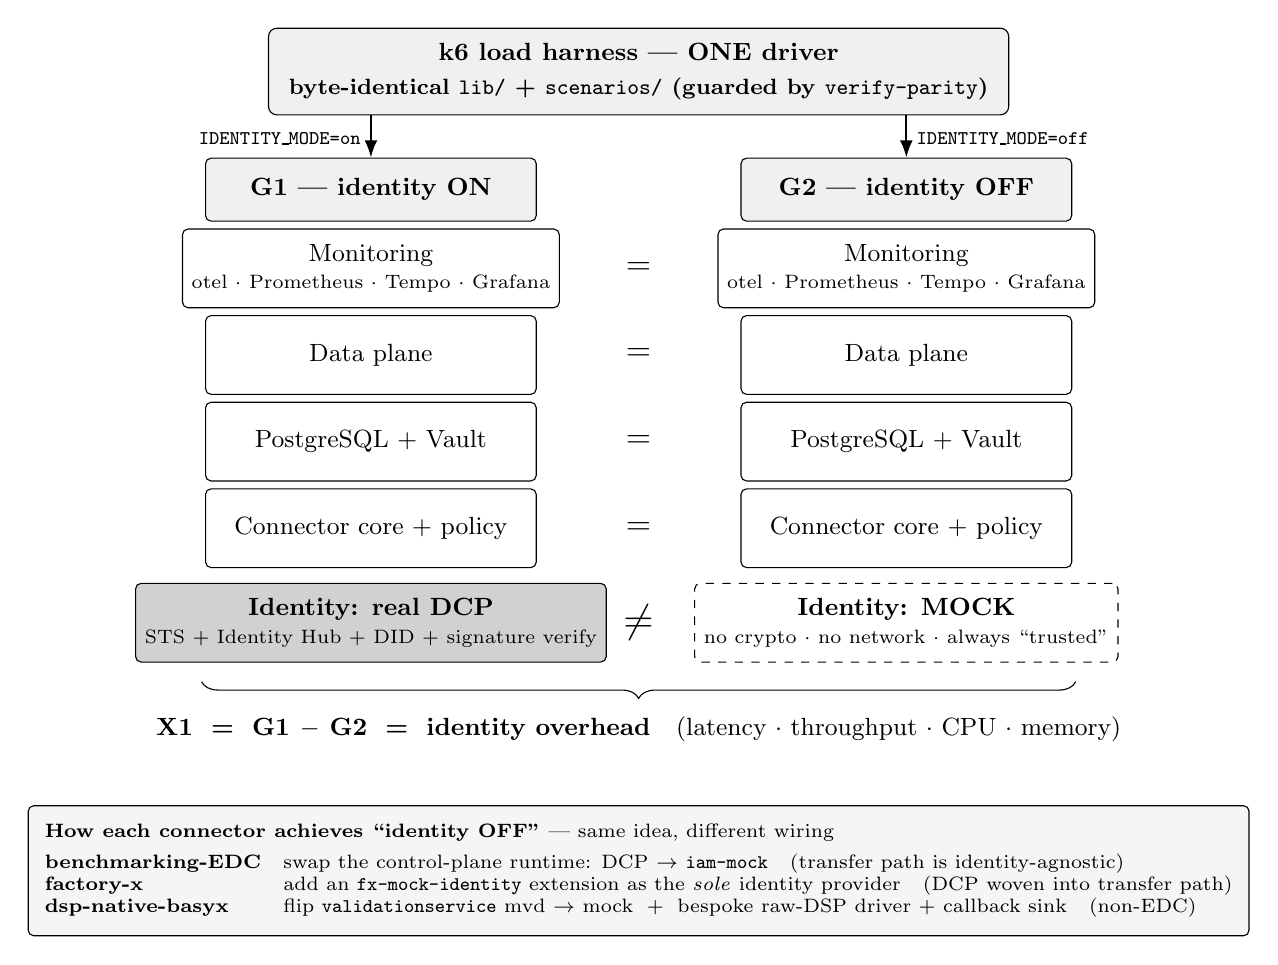
\begin{tikzpicture}[
  layer/.style   = {draw, rounded corners=2pt, minimum width=4.2cm, minimum height=1.0cm,
                    align=center, font=\small, fill=white},
  idon/.style    = {layer, fill=black!18},
  idoff/.style   = {layer, dashed, fill=white},
  goal/.style    = {draw, rounded corners=2pt, minimum width=4.2cm, minimum height=0.8cm,
                    align=center, font=\small\bfseries, fill=black!6},
  harness/.style = {draw, rounded corners=3pt, minimum width=9.4cm, minimum height=1.1cm,
                    align=center, font=\small\bfseries, fill=black!6},
  arr/.style     = {-{Latex[length=2.2mm]}, thick},
  eq/.style      = {font=\large},
]

% ---- the single driver ------------------------------------------------------
\node[harness] (h) at (0,7.6)
  {k6 load harness --- ONE driver\\[1pt]
   \footnotesize byte-identical \texttt{lib/} + \texttt{scenarios/} (guarded by \texttt{verify-parity})};

% ---- the two goals ----------------------------------------------------------
\node[goal] (gL) at (-3.4,6.1) {G1 --- identity ON};
\node[goal] (gR) at ( 3.4,6.1) {G2 --- identity OFF};

\draw[arr] (h.south -| gL) -- node[left,  font=\scriptsize, pos=0.55] {\texttt{IDENTITY\_MODE=on}}  (gL.north);
\draw[arr] (h.south -| gR) -- node[right, font=\scriptsize, pos=0.55] {\texttt{IDENTITY\_MODE=off}} (gR.north);

% ---- left stack (ON) --------------------------------------------------------
\node[layer] (lMon)  at (-3.4,5.1) {Monitoring\\[-1pt]\scriptsize otel $\cdot$ Prometheus $\cdot$ Tempo $\cdot$ Grafana};
\node[layer] (lDP)   at (-3.4,4.0) {Data plane};
\node[layer] (lPV)   at (-3.4,2.9) {PostgreSQL + Vault};
\node[layer] (lCore) at (-3.4,1.8) {Connector core + policy};
\node[idon]  (lId)   at (-3.4,0.6) {\textbf{Identity: real DCP}\\[-1pt]\scriptsize STS + Identity Hub + DID + signature verify};

% ---- right stack (OFF) ------------------------------------------------------
\node[layer] (rMon)  at ( 3.4,5.1) {Monitoring\\[-1pt]\scriptsize otel $\cdot$ Prometheus $\cdot$ Tempo $\cdot$ Grafana};
\node[layer] (rDP)   at ( 3.4,4.0) {Data plane};
\node[layer] (rPV)   at ( 3.4,2.9) {PostgreSQL + Vault};
\node[layer] (rCore) at ( 3.4,1.8) {Connector core + policy};
\node[idoff] (rId)   at ( 3.4,0.6) {\textbf{Identity: MOCK}\\[-1pt]\scriptsize no crypto $\cdot$ no network $\cdot$ always ``trusted''};

% ---- "everything equal except identity" ------------------------------------
\node[eq] at (0,5.1) {$=$};
\node[eq] at (0,4.0) {$=$};
\node[eq] at (0,2.9) {$=$};
\node[eq] at (0,1.8) {$=$};
\node[font=\Large\bfseries] at (0,0.6) {$\neq$};

% ---- the delta --------------------------------------------------------------
\draw[decorate, decoration={brace, mirror, amplitude=6pt}] (-5.55,-0.15) -- (5.55,-0.15);
\node[font=\small] at (0,-0.75)
  {\textbf{X1 \;=\; G1 $-$ G2 \;=\; identity overhead}\quad(latency $\cdot$ throughput $\cdot$ CPU $\cdot$ memory)};

% ---- per-connector technique strip -----------------------------------------
\node[draw, rounded corners=2pt, fill=black!4, font=\scriptsize, inner sep=6pt] at (0,-2.55)
  {\begin{tabular}{@{}l@{\hskip 8pt}l@{}}
     \multicolumn{2}{@{}l@{}}{\textbf{How each connector achieves ``identity OFF''} --- same idea, different wiring}\\[3pt]
     \textbf{benchmarking-EDC} & swap the control-plane runtime: DCP $\rightarrow$ \texttt{iam-mock}\quad(transfer path is identity-agnostic)\\
     \textbf{factory-x}        & add an \texttt{fx-mock-identity} extension as the \emph{sole} identity provider\quad(DCP woven into transfer path)\\
     \textbf{dsp-native-basyx} & flip \texttt{validationservice} mvd $\rightarrow$ mock \;+\; bespoke raw-DSP driver + callback sink\quad(non-EDC)\\
   \end{tabular}};

\end{tikzpicture}
\end{document}
